\chapter{Экспериментальный раздел}
В текущем разделе будет поставлена цель эксперимента, проведён сам эксперимент и сделаны соответствующие выводы. 

\section{Технические характеристики}

Технические характеристики устройства, на котором выполнялось тестирование, следующие.

\begin{itemize}
	\item Операционная система: Arch Linux \cite{oswind} x86\_64.
	\item Память: 48 GiB.
	\item Процессор: 11th Gen Intel® Core™ i5-1135G7 @ 2.40GHz \cite{intel}.
	\item 4 физических ядра и 8 логических ядра.
\end{itemize}

Тестирование проводилось на ноутбуке, включенном в сеть электропитания. Во время тестирования ноутбук был нагружен только встроенными приложениями окружения, а также непосредственно системой тестирования.


\section{Постановка эксперимента 1} 

\subsection{Цель эксперимента}
Цель эксперимента -- узнать зависимость количества времени на обработку кадра от количества потоков.

Гипотеза - чем больше потоков, тем лучше. ПРи этом отключена всякая параллельность задач на видеокарте, разговор идет только про количество потоков запуска функции.

На рисунке \ref{img:e4} приведен график зависимости количества миллисекунд от количества потоков.

\begin{figure}[H]
	\begin{center}
		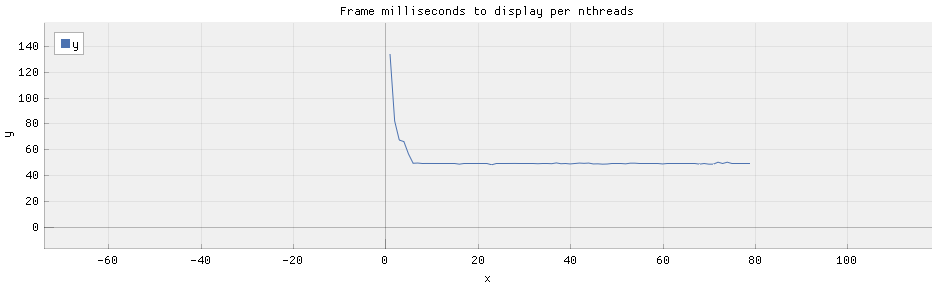
\includegraphics[scale=0.60]{img/avg_time_focused.png}
	\end{center}
	\captionsetup{justification=centering}
	\caption{Зависимость количества миллисекунд (по y) от количества потоков (по x). }
	\label{img:e4}
\end{figure}


\section{Постановка эксперимента 1} 

\subsection{Цель эксперимента}
Цель эксперимента -- узнать зависимость количества времени на обработку кадра от количества потоков.

Гипотеза - чем больше потоков, тем лучше. ПРи этом отключена всякая параллельность задач на видеокарте, разговор идет только про количество потоков запуска функции.

На рисунке \ref{img:e4} приведен график зависимости количества миллисекунд от количества потоков.

\begin{figure}[H]
	\begin{center}
		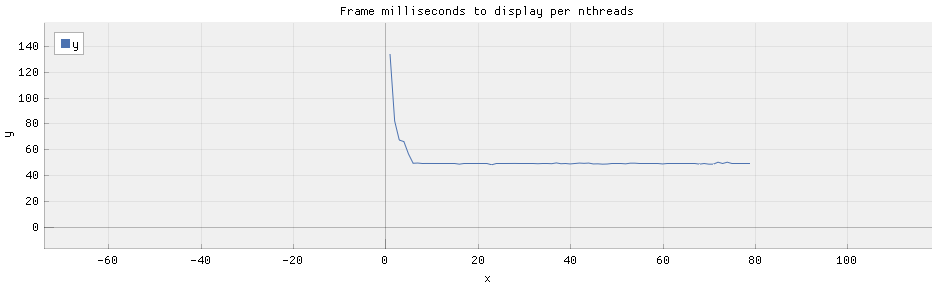
\includegraphics[scale=0.60]{img/avg_time_focused.png}
	\end{center}
	\captionsetup{justification=centering}
	\caption{Зависимость количества миллисекунд (по y) от количества потоков (по x). }
	\label{img:e4}
\end{figure}


\section*{Вывод}

В результате эксперимента было выявлено, что оптимизированный алгоритм обратной трассировки лучей на самом деле дает выигрыш во времени, так как требует меньшего количества лучей для построения сцены. Кроме того, расчитанные аналитическим способом результаты были подтверждены на практике.

